\documentclass[11pt]{article}
\usepackage[dvipsnames, table]{xcolor}
\usepackage{times}
\usepackage{amsmath,amsthm,amssymb,setspace,enumitem,epsfig,titlesec,verbatim,array,eurosym,multirow}
\usepackage[sort&compress,numbers]{natbib}
\usepackage[footnotesize,bf]{caption}
\usepackage[margin=2.5cm, includefoot, footskip=30pt]{geometry}
\usepackage{standalone}
\usepackage{tikz}
\usepackage{subcaption}
\usepackage{hyperref}
\usepackage{tabularx}
\usepackage{booktabs}
\usepackage{blkarray}
\usepackage[ruled,vlined]{algorithm2e}
\smallskip % Erlaubt kleine Abstaende zwischen Paragraphen, falls es dem Seitenlayout hilft
\renewcommand{\baselinestretch}{1.15}
\usepackage{tikz}
\usetikzlibrary{arrows}
\usepackage{minitoc}
\usepackage{graphicx}
\usepackage{hyperref}
\usepackage{subcaption}
\usepackage{multirow}
\usepackage{multicol}
\usepackage{standalone}
\usepackage{makecell}

\newcommand{\nikoleta}[1]{\textcolor{orange}{\textbf{NG}: #1}}
\newcommand{\christian}[1]{\textcolor{blue}{\textbf{CH}: #1}}

\newtheoremstyle{plainCl1}% name
{12pt}%      Space above, empty = 'usual value'
{12pt}%      Space below
{\it}% 	   Body font
{}%         Indent amount (empty = no indent, \parindent = para indent)
{\bfseries}% Thm head font
{}%        Punctuation after thm head
{\newline}% Space after thm head: \newline = linebreak
{}%         Thm head spec

\theoremstyle{plainCl1}
\newtheorem{theorem}{Theorem}
\newtheorem{lemma}{Lemma}
\newtheorem{corollary}{Corollary}
\newtheorem{proposition}{Proposition}


\newtheoremstyle{plainCl2}% name
{12pt}%      Space above, empty = 'usual value'
{12pt}%      Space below
{}% 	   Body font
{}%         Indent amount (empty = no indent, \parindent = para indent)
{\bfseries}% Thm head font
{}%        Punctuation after thm head
{\newline}% Space after thm head: \newline = linebreak
{}%         Thm head spec

\theoremstyle{plainCl2}
\newtheorem*{definition}{Definition}



\def\wsls{\texttt{WSLS}}
\def\tft{\texttt{TFT}}
\def\gtft{\texttt{GTFT}}
\def\allc{\texttt{ALLC}}
\def\alld{\texttt{ALLD}}
\def\alt{\texttt{Alternator}}



\titleformat{\section}{\sffamily \fontsize{12}{15}\bfseries}{\thesection}{0.4em}{}
\titleformat{\subsection}{\sffamily\fontsize{11}{15}\bfseries}{\thesubsection}{0.4em}{}
\renewcommand{\thefigure}{S\arabic{figure}}


\title{~\\[-1.5cm]{\sffamily \Large Revision notes}\\[-0.3cm]}

\date{\empty}

\begin{document}


\section{Related Literature}

There is now an extensive body of literature on repeated games and the
strategies used by players in these games. This literature has introduced
various strategies that succeed in evolutionary simulations and/or computer
tournaments. Moreover, it has explored the conditions under which cooperation
can emerge as an outcome, and the strategies that can facilitate this.

One classification of repeated game strategies is that of finite memory
strategies. These strategies base decisions on the outcomes of the last \(n\)
rounds. The most well-studied among these is the set of memory-one strategies,
where decisions are made solely based on the previous turn. This set has
been used to introduce concepts such as zero-determinant strategies, as well as
partner and rival strategies. Zero-determinant strategies are those that can
enforce a linear relationship between the players' payoffs. Partner strategies
are Nash strategies that maintain full cooperation when used by both players,
even in the presence of implementation errors. Rival strategies ensure that the
co-player never obtains a higher payoff than the rival does, regardless of the
co-player's strategy.

In the context of our paper, the most relevant literature is the recent work on
higher memory strategies and the characterization of Nash equilibria in repeated
games. In this section, we cover a selection of these papers and highlight the
differences between our work and theirs. \\

\noindent
{\bf The work of Ueda~\cite{ueda:RSOP:2021, Ueda:ORF:2022}.}
There has been considerable focus on zero-determinant (ZD) strategies in
repeated games. ZD strategies were introduced in \cite{press:PNAS:2012} and
represented a significant breakthrough, as they can enforce a linear
relationship between players' payoffs.

The work of Ueda \cite{ueda:RSOP:2021} specifically focuses on memory-2
ZD strategies. Ueda demonstrates that Akin's Lemma \cite{akin:EGADS:2016} can be
generalized to any memory size and uses this generalization to characterize ZD
strategies in the memory-two space. He focuses on a subset of these ZD
strategies, which he calls variants of tit-for-tat. Ueda also shows that all ZD
strategies in the space of memory-\(n\) can be characterized. In a subsequent
work \cite{Ueda:ORF:2022}, among other results, Ueda examines these
tit-for-tat-like ZD strategies and demonstrates that they can be generalized to
any \(n\).

In our work, we achieve similar results to Ueda regarding the generalization of
Akin's Lemma (our SI Lemma 1) and the characterization of zero-determinant
strategies (our SI Equation 22). However, we differentiate from these studies in
several key ways:

\begin{itemize} 
\item We characterize additional zero-determinant strategies,
specifically delayed tit-for-tat and delayed generous tit-for-tat strategies,
which were not characterized in Ueda's work.
\end{itemize}


\noindent
{\bf The work of Murase and Baek~\cite{murase:SciRep:2020, Murase:PLoSCompBio:2023a}.}
The work of \cite{murase:SciRep:2020, Murase:PLoSCompBio:2023a} investigates
strategies with higher memory using numerical simulations. Specifically, they
explore the space of pure memory-two and memory-three strategies and classify
which of these strategies are partners and which are rivals. More importantly,
the work of \cite{murase:SciRep:2020} introduces a new class of strategies
called friendly rivals. These strategies have the properties of rivals; however,
they also provide an incentive to form mutual cooperation. The authors show that
this class can only be achieved if at least two rounds of memory are considered.

In \cite{Murase:PLoSCompBio:2023a}, the authors examine whether these strategies
would be learned in an evolutionary setting, similar to our work where we
investigate the evolutionary dynamics of reactive strategies. They found that
friendly rivals play a minor role, as partner strategies are sufficient to foster
cooperation.

\begin{itemize}
\item In our work, we classify the reactive strategies that are partners for a given
memory, but we also do this for all strategies, both stochastic and
deterministic. We demonstrate that this is an analytical result.
\end{itemize}

\noindent
{\bf The work of McAvoy and Nowak~\cite{mcavoy:PRSA:2019}.}
The work of McAvoy and Nowak~\cite{mcavoy:PRSA:2019} investigates the feasible
payoffs of strategies in repeated games. Building on the concept of ZD
strategies, where it was shown that one strategy can control the payoff space,
they explore whether other such classes exist. However, instead of focusing on
memory-\(n\) strategies, they introduce a new class called reactive learning
strategies. These strategies have infinite memory because they gradually modify
their propensity to take certain actions based on the opponent's past actions,
which is why they are termed reactive. McAvoy and Nowak focus on the feasible
payoff space and demonstrate that if a player uses a memory-one strategy, they
could transition to an equivalent reactive learning strategy, which would
constrain the co-player's payoffs even more.

The authors show that the payoff space is convex in memory-one strategies, which
means that it is sufficient to check only pure memory-one strategies to
understand if that a given memory-one strategy is Nash. We demonstrate a similar
result with pure self-reactive strategies when the player considers reactive
strategies. However, our result work for any \(n\). Moreover, our work is
focused on deriving conditions for Nash equilibria, a question that McAvoy and
Nowak did not investigate. \\


\noindent
{\bf The work of Stewart and Plotkin~\cite{stewart:scientific:2016}.}
The authors investigate higher memory strategies in public goods games. Their
results focus on memory-\(n\) strategies, specifically on
counting strategies. This is because, in public goods games, payoffs
depend on the number of cooperators in the group. The authors retrieve a series
of analytical results, characterizing when strategies are ``robust''.

In the following, we explain what it means for a strategy to be ``robust''. In
an evolutionary process, when considering the low mutation limit, only two types
can exist in the population. The key question is: what is the probability that a
single mutant will fix? This depends on the payoff that individuals receive in
the current state of the population compared to the resident strategy. If the
mutant's payoff is higher, it will fix. If the resident population consistently
has a greater payoff than any mutant, then the resident strategy is resistant to
invasion and is termed "robust," as described by Stewart and Plotkin.

The authors determine the conditions under which nice strategies and strategies
that defect after mutual defection are robust. They also calculate the relative
volumes of robust cooperation, the absolute volume of robust cooperative
strategies divided by the total volume of robust cooperators and defectors, and
compare this to the relative volume of defectors. They find that the volume of
robust cooperation increases as memory increases. This is very similar to our
results regarding the proportion partner and defective Nash strategies.

However, this result does not necessarily explain the course of evolution. Even
though the volume of these strategies is larger and more of them exist in this
space, it does not mean that running an evolutionary process will increase the
average cooperation rate. The authors do not provide conditions in the same form
as we do regarding when a given strategy is Nash. The considerations they offer
still depend on the strategies that the players use.

%% DEFECTING STRATEGIES: Donation Game %%

\section{Reactive defecting Nash strategies in the donation game}\label{section:defecting_donation_game}

In the previous sections, we characterized reactive partner strategies for the
special case of the donation game and the general prisoner's dilemma. In the
following section, we apply the same methods to characterize defecting Nash
equilibria. For the case of reactive-1 strategies, we obtain the following
characterization.

%% DEFECTING STRATEGIES: Reactive-1 Donation Game %%

\begin{theorem}[Reactive-1 defecting Nash strategies in the donation game]
\label{theorem:reactive_one_defecting_strategies}
A reactive-1 strategy $\mathbf{p}$ is a defecting Nash strategy if and only if
its entries satisfy the conditions

\begin{equation}
  \begin{array}{rcl}
    p_{C} \le  \frac{c}{b} \qquad \text{ and } \qquad  p_{D} \!=\! 0.
\end{array}
\end{equation}
\end{theorem}


%% DEFECTING STRATEGIES: Reactive-2 Donation Game %%

\begin{theorem}[Reactive-2 defecting Nash strategies in the donation game]
\label{theorem:reactive_two_defecting_strategies}
A reactive-2 strategy $\mathbf{p}$ is a defecting Nash strategy if and only if
its entries satisfy the conditions

\begin{equation}\label{eq:defecting_conditions_two}
  p_{CC} \le \frac{c}{b}, \qquad \displaystyle \frac{p_{CD} \!+\! p_{DC}}{2} \le \frac{c}{2b}, \qquad p_{DD} = 0.
\end{equation}
\end{theorem}

%% DEFECTING STRATEGIES: Reactive-3 Donation Game %%

\begin{theorem}[Reactive-3 defecting Nash strategies in the donation game]
\label{theorem:reactive_three_defecting_strategies}
A reactive-3 strategy $\mathbf{p}$ is a defecting Nash strategy if and only if
its entries satisfy the conditions

\begin{align}\label{eq:defecting_conditions_three}
  \begin{split}
  p_{CCC} & \le \frac{c}{b} \\
  \frac{p_{CDC} + p_{DCD}}{2} & \leq \frac{1}{2} \cdot \frac{c}{b} \\
  \frac{p_{CCD} + p_{CDC} + p_{DCC}}{3} & \leq \frac{2}{3} \cdot \frac{c}{b} \\
  \frac{p_{CDD} + p_{DCD} + p_{DDC}}{3} & \leq \frac{1}{3} \cdot \frac{c}{b} \\
  \frac{p_{CCD} + p_{CDD} + p_{DCC} + p_{DDC}}{4}  & \leq \frac{1}{2} \cdot \frac{c}{b}  \\
  p_{DDD} & = 0.
  \end{split}
\end{align}

\end{theorem}

\noindent
We repeat the same analysis for reactive counting strategies. We obtain the
following results.

%% DEFECTING STRATEGIES: Reactive-2 Counting Donation Game %%

\begin{theorem}[Reactive-2 defecting Nash counting strategies in the donation game]
\label{theorem:reactive_two_defecting_counting_strategies}
A reactive-2 counting strategy $\mathbf{r}$ is a defecting Nash strategy if and only if
its entries satisfy the conditions

\begin{equation}\label{eq:defecting_conditions_two_counting}
  r_{2} \le \frac{c}{b}, \qquad \displaystyle r_{1} \le \frac{1}{2} \cdot \frac{c}{b}, \qquad r_{0} = 0.
\end{equation}
\end{theorem}

%% DEFECTING STRATEGIES: Reactive-3 Counting Donation Game %%

\begin{theorem}[Reactive-3 defecting Nash counting strategies in the donation game]
\label{theorem:reactive_three_defecting_counting_strategies}
A reactive-3 counting strategy $\mathbf{r}$ is a defecting Nash strategy if and only if
its entries satisfy the conditions

\begin{equation}\label{eq:defecting_conditions_three_counting}
  r_{3} \le \frac{c}{b}, \qquad r_{2} \leq\frac{2}{3} \cdot \frac{c}{b}, \qquad
  r_{1} \leq\frac{1}{3} \cdot \frac{c}{b}, \qquad
  r_{0} = 0.
\end{equation}
\end{theorem}

\noindent
We can observe that for each value of \(n\), the left-hand side of the
conditions for cooperative and defective Nash are the same. Moreover, we see
that, for a low cost-to-benefit ratio, the right-hand side of the defective Nash
conditions is always strictly smaller than those of the cooperative Nash
conditions. This means that within the space of feasible strategies, the volume
of partner strategies is larger than the volume of defective Nash strategies. We
also verify these analytical results numerically
(Figure~\ref{fig:siFigDefectiveCooperativeNash}), and we also show that as memory increases,
the number of cooperative and defective Nash strategies decreases, as the
strategy spaces are larger. However, the decrease is more prominent in the case
of defective Nash.

\begin{figure}[h]
  \centering
  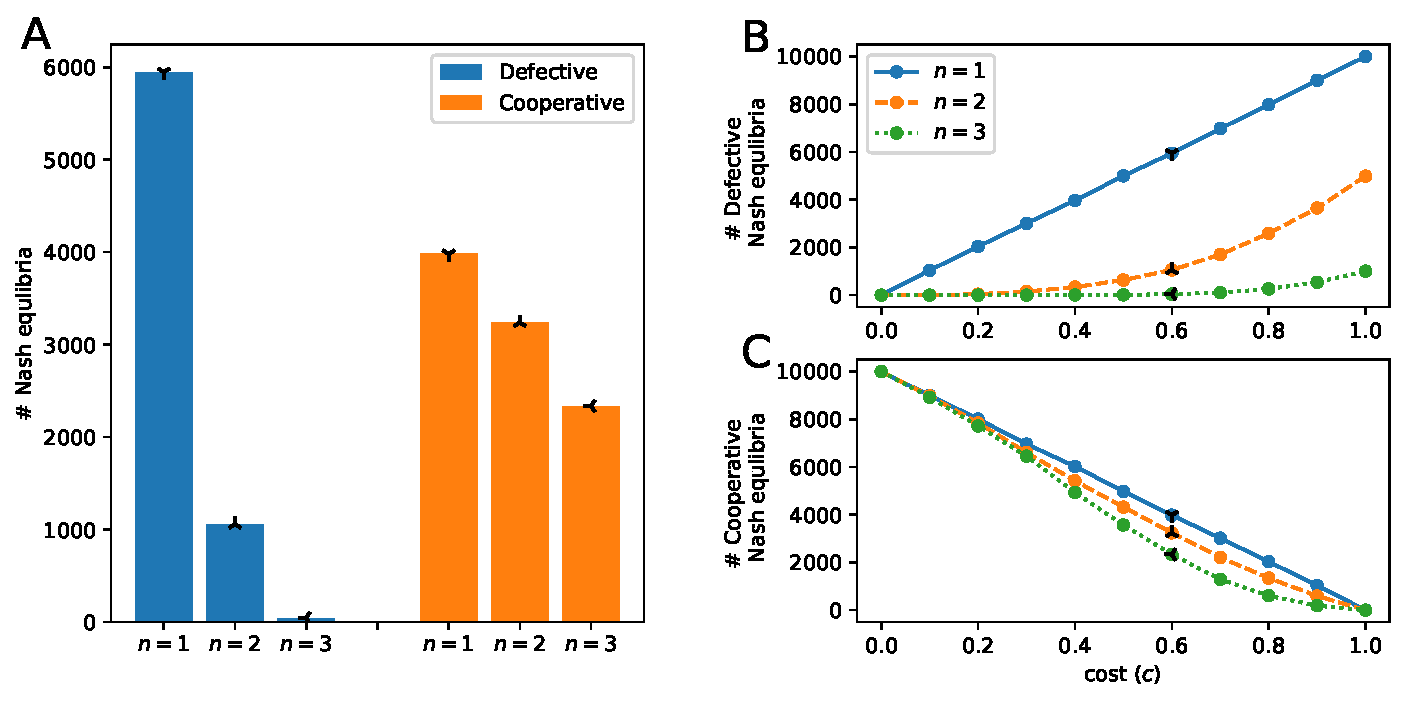
\includegraphics[width=\textwidth]{../../figures/siFig1.pdf}
  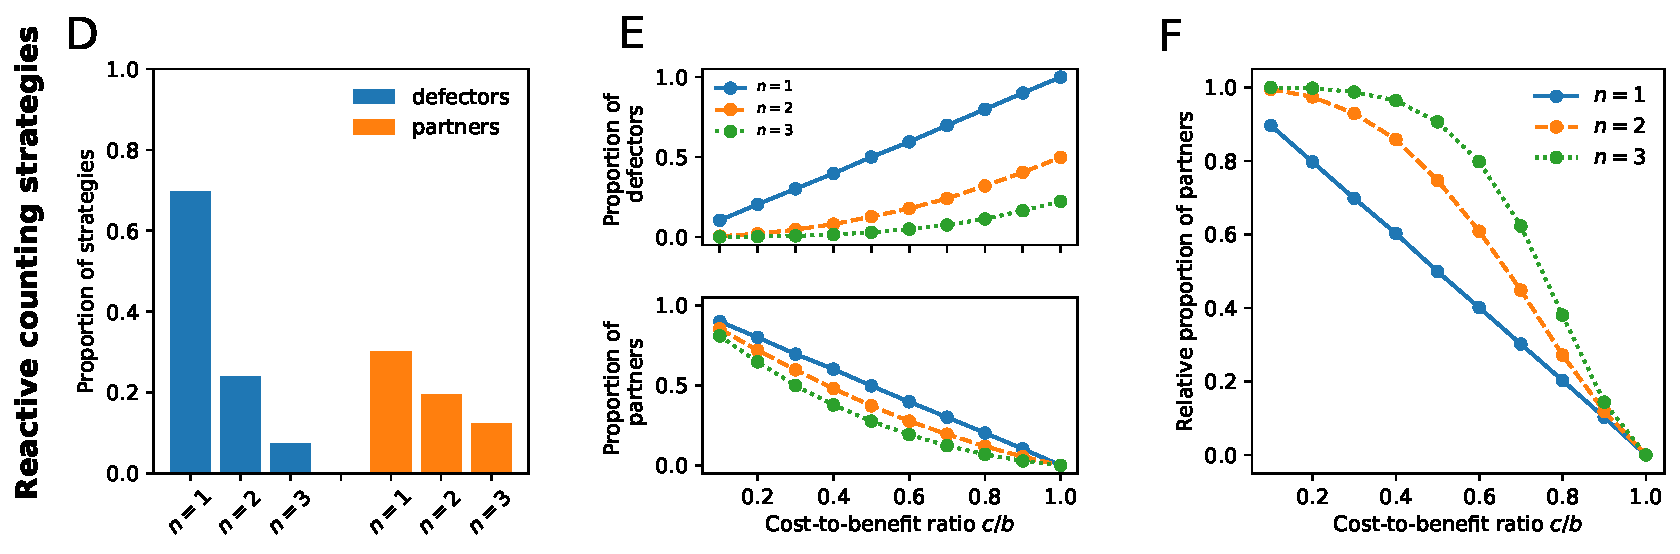
\includegraphics[width=\textwidth]{../../figures/siFig1Counting.pdf}
  \caption{
  \textbf{Proportions of cooperative and defective Nash.}
We draw \(10^4\) random strategies from the feasible space of strategies and
create two copies of each strategy. For one copy, we set the probability of
cooperating after full cooperation of the co-player to 1. For the second copy,
we set the probability of cooperating after full defection of the co-player to
0. We then check if either copy is Nash: cooperative for the first copy and
defective for the second. We set the benefit of cooperation to \(b = 1\).
{\bf A, D,} We plot the results for a given value of cost, \(c = 0.5\). We do
this for reactive strategies and reactive counting strategies. For \(n=1\), we
can see the number of defective equilibria is higher than that of the
cooperative. However, as we increase \(n\), this is no longer true. The number
of defective Nash decreases drastically. The number of partner strategies does
as well, but to a lesser extent.
{\bf B, E,} We plot the proportion of equilibria over different values of cost, for reactive
and reactive counting strategies. As the cost increases, so does the
proportion of defective equilibria, and the opposite is true for cooperative. As
memory increases, we observe again a significant drop in the proportion of
defective strategies, whereas there is a small decrease in the cooperative
strategies. 
{\bf C, D,} We plot the relative proportion of cooperative Nash strategies. For
this, we consider the sum of cooperative and defecting Nash strategies for each
memory size and plot the number of cooperative Nash strategies over the total
sum. This proportion increases as memory size increases.
}\label{fig:siFigDefectiveCooperativeNash}
\end{figure}


%%%%%%%%%%%%%%%%%%%%%%%%%%%
%% Evolutionary Simulations  %%
%%%%%%%%%%%%%%%%%%%%%%%%%

\newpage
\section{Evolutionary Simulations}

We repeated the evolutionary analysis of Figure 4 of the main text. This time,
for panels \textbf{A} and \textbf{B}, we ran twenty independent simulations. We
did this to check that the results, specifically the mean most abundant
strategies, do not change.

\begin{figure}[tbhp]
    \centering
    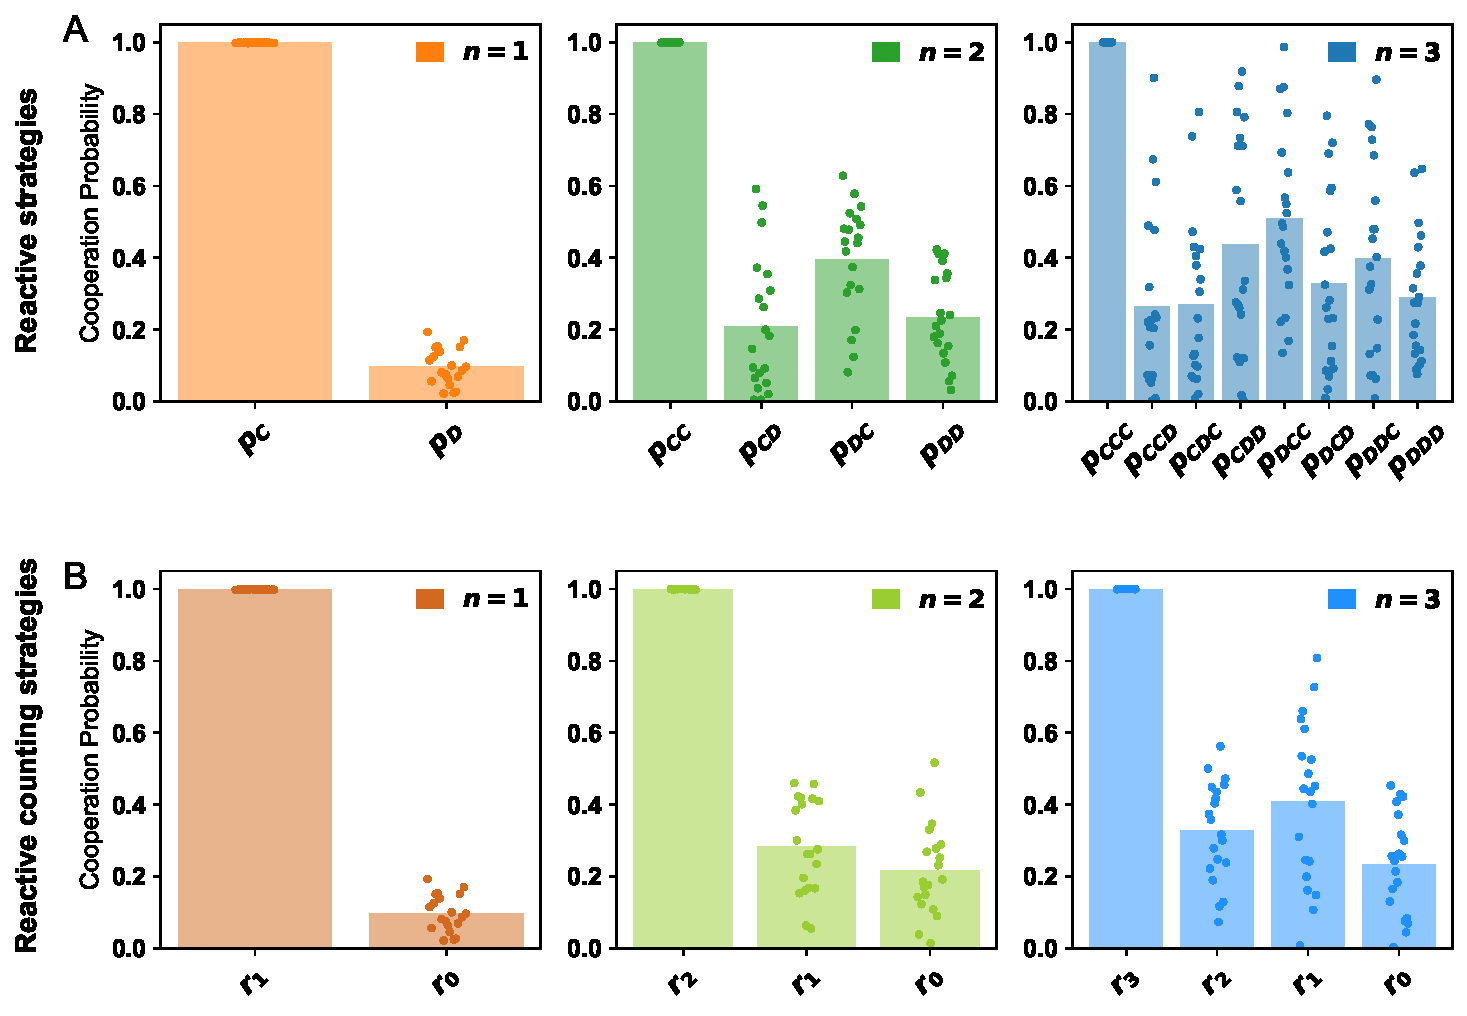
\includegraphics[width=\textwidth]{../../figures/siFig3AbundantStrategies.pdf}
    \caption{\textbf{Evolutionary dynamics of reactive-$n$ strategies: Most abundant strategies.}
    The same process as that in the paper for Figure 4 is used, with the same
    parameters. Simulations are based on a donation game with \(b\!=\!1\),
    \(c\!=\!0.5\), a selection strength \(\beta\!=\!1\), and a population size
    \(N\!=\!100\). For \(n\) equal to 1 and 2, simulations
    are run for \(T\!=\!10^7\) time steps. For \(n\!=\!3\), we use \(T\!=\!2 \cdot
    10^7\) time steps. This time, we run twenty independent simulations instead of
    ten.
    }\label{fig:siFigAbundantStrategies}
\end{figure}

\subsection{Invasion Analysis}

One question that arises is which of these top strategies are partner
strategies, and why some partner strategies are selected more than others. For
example, in the case of reactive-1 strategies, we consider a reactive strategy
to be partner if \((p_{C} > 0.95)\) and \((p_{D} < \frac{c}{b})\). Here, we
observe strategies with \((p_{D} \approx 0.1)\) and not those closer to the
boundary. The reason for this is explained by
Figure~\ref{fig:InvasionAnalysisReactive1}. \\


\begin{figure}[tbhp]
  \centering
  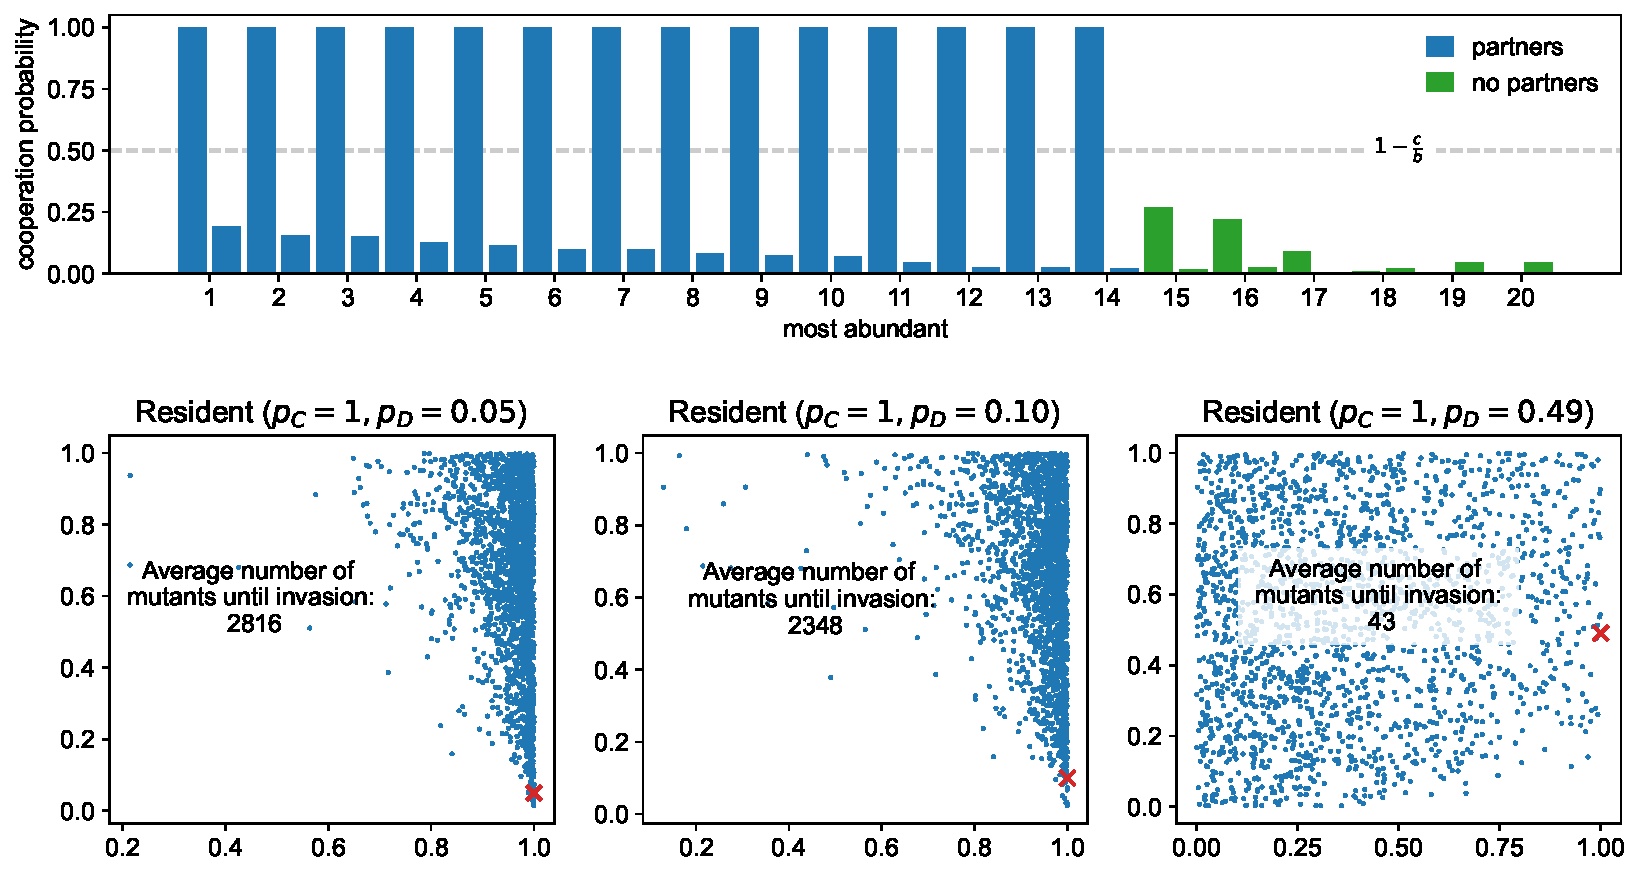
\includegraphics[width=\textwidth]{../../figures/siFigInvasionR1.pdf}
  \caption{\textbf{Invasion analysis for reactive-1.}
  {\bf A,} The twenty most abundant reactive-1 strategies of
  Figure~\ref{fig:siFigAbundantStrategies}. We observe that all twenty of them
  are partner strategies, and that all have a very low \(p_D\), typically less
  than 0.2.
  {\bf B,} We perform an invasion analysis. Namely, we select one resident and introduce
  mutants until a mutant becomes the new resident. We record how many mutants
  were introduced until this happens. We do this \(10^3\) times and report the
  average number of mutants over all the simulations. We consider three different
  residents. For each, we report the average number of mutants until invasion and
  the mutants that invaded as well (scatter points). We observed that a resident with a very low \(p_D\) is more resistant to
  invasion, which explains why we observe that the most abundant strategies have a
  low \(p_D\). 
  {\bf C,} To explain why a low \(p_D\) leads to more resistance to invasion, we
  look at the expected payoffs of each resident when when \(k\) \alld{}
  mutants try to invade. We can see that for the
  far-left resident, the expected payoff is almost always strictly higher than
  that of the \alld{} mutants; only when there are 99 mutants is the payoff the same.}\label{fig:InvasionAnalysisReactive1}
\end{figure}

\noindent
A similar question arises for reactive-2 strategies. More specifically, why is
it that we observe partner strategies where \(p_{CD}\) is almost always strictly
lower than \(p_{DC}\)? Why are these partners chosen more often by the
evolutionary process? \\


\begin{figure}[tbhp]
  \centering
  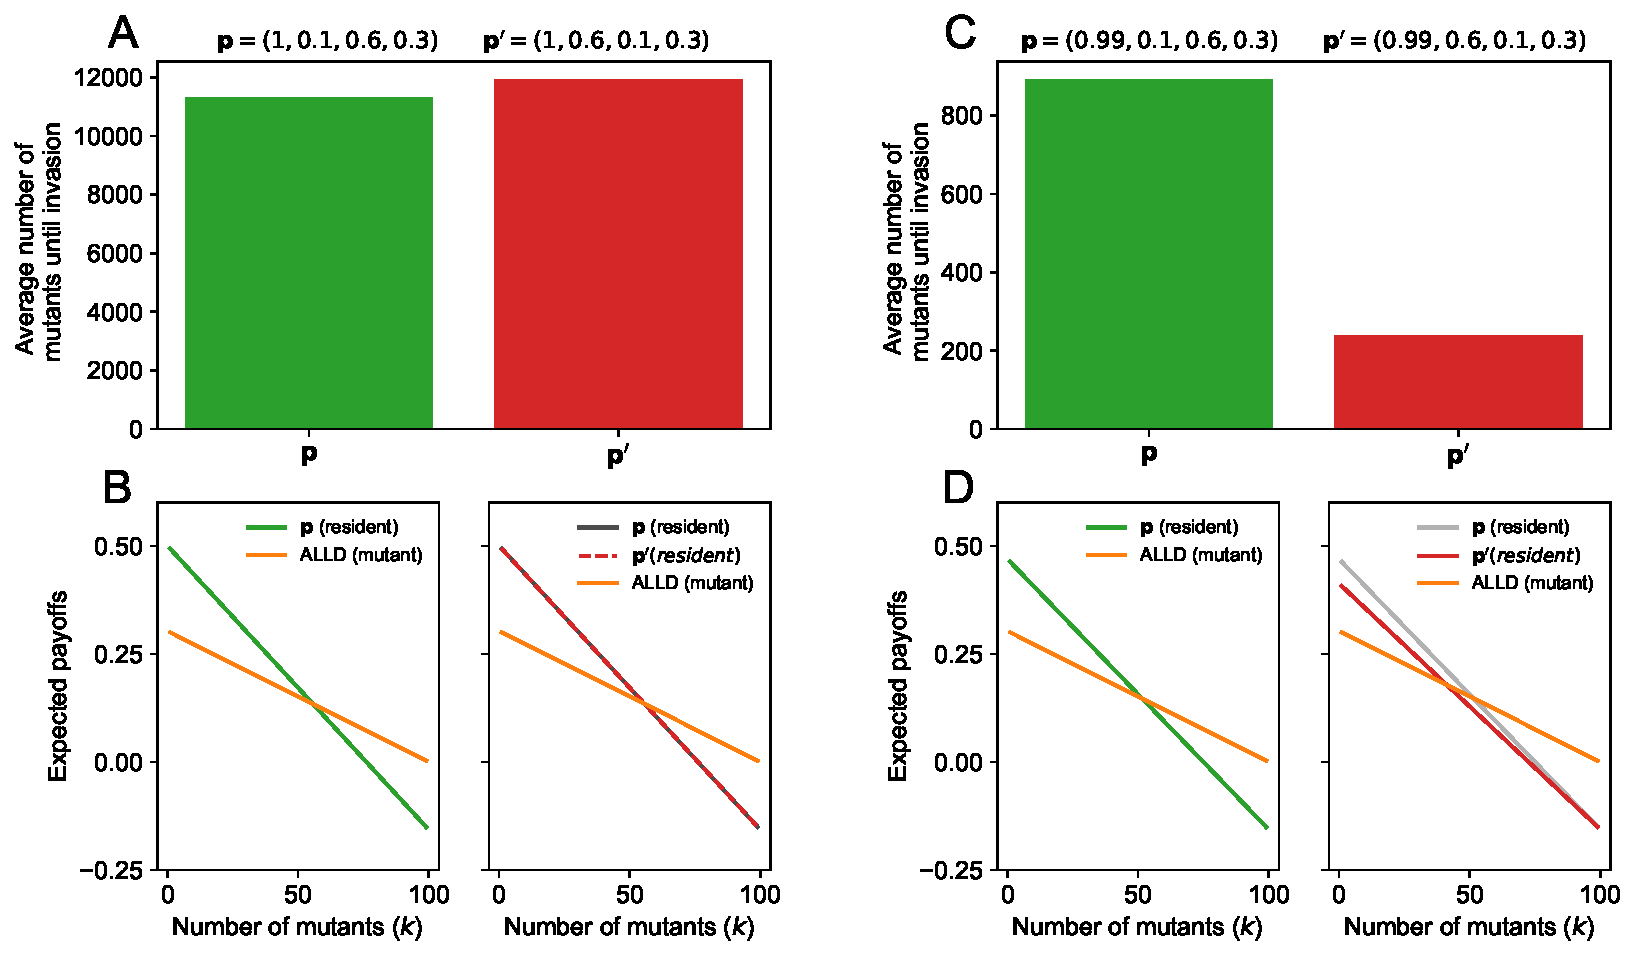
\includegraphics[width=\textwidth]{../../figures/siFigInvasionR2.pdf}
  \caption{\textbf{Invasion analysis for reactive-2.}
  {\bf A,}  We repeated the same analysis for the case of reactive-2 strategies. The
  twenty top-performing strategies are partner strategies. We observe that
  the partner strategies selected by the evolutionary process almost always have a
  smaller \(p_{CD}\) than \(p_{DC}\) and a low \(p_{DD}\).
  {\bf B,} We already know why residents with low \(p_{DD}\) are more abundant. To
  understand the entries \(p_{CD}\) and \(p_{DC}\), we will consider two example
  strategies: \(\mathbf{p} = (0.99, 0.10, 0.60, 0.30)\) and \(\mathbf{p'} = (0.99,
  0.60, 0.10, 0.30)\). We perform an invasion analysis when either \(\mathbf{p}\)
  or \(\mathbf{p'}\) are the resident, and we introduce mutants until a mutant
  becomes the new resident. We repeat this process \(10^4\) times and report the
  average time until invasion over all the repetitions. We observe that
  \(\mathbf{p'}\) is invaded much faster.
  {\bf C,} We calculate the expected payoffs of \(\mathbf{p}\) and \(\mathbf{p'}\)
  when \(k\) \alld{} mutants are present. We observe that the self-payoffs
  of the strategies are different, which in turn means that fewer \alld{}
  mutants are required for \alld{}  to achieve a higher payoff compared to
  \(\mathbf{p'}\).
  }\label{fig:InvasionAnalysisReactive2}
\end{figure}

\begin{figure}[tbhp]
  \centering
  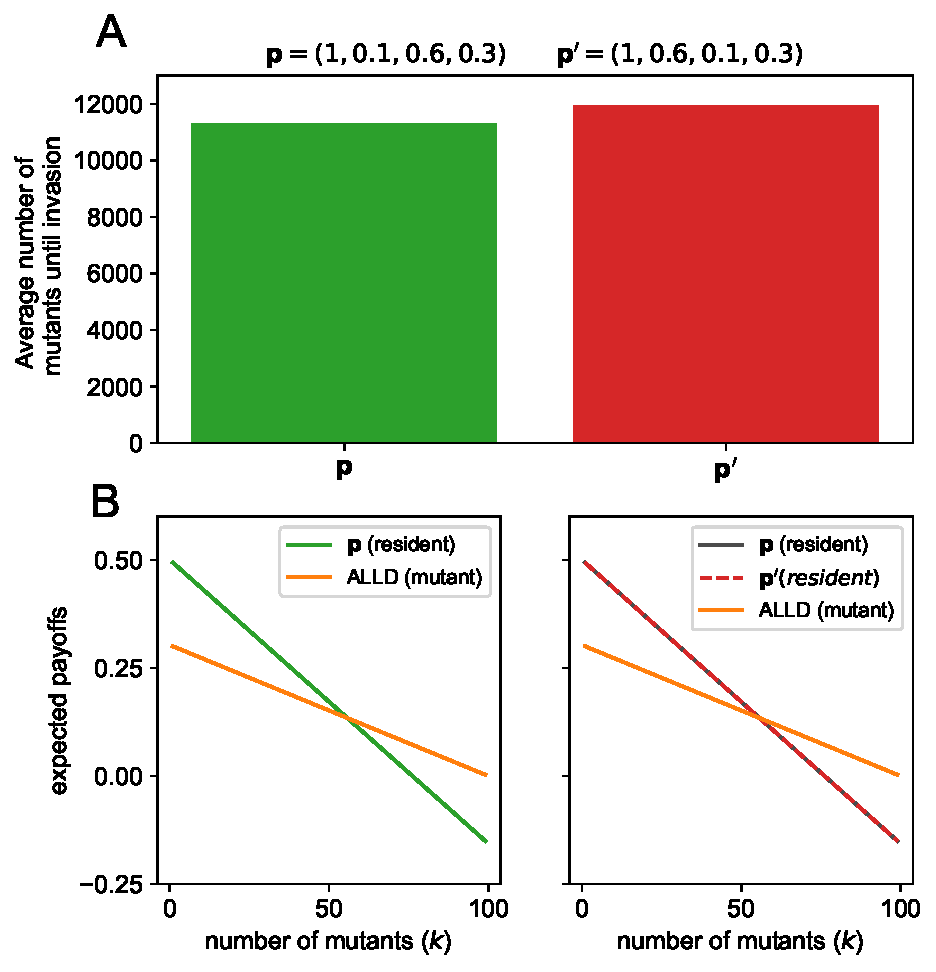
\includegraphics[width=.65\textwidth]{../../figures/siFigInvasionR2ForPCCone.pdf}
  \caption{\textbf{Invasion analysis for reactive-2 with $p_{CC}=1$.}
  We repeat the analysis described in Figure~\ref{fig:InvasionAnalysisReactive2}
  {\bf B} and {\bf C}, but this time we consider the case where \(p_{CC} = p'_{CC}
  = 1\). In {\bf A}, we plot the average number of mutants until invasion for both
  strategies, and in {\bf B}, we plot the expected payoffs of the strategies when
  \(k\) \alld{} mutants are present in the population, while \(N-k\) are the
  resident strategy. Both strategies now have the same average number of mutants
  until invasion and the same expected payoffs.
  }\label{fig:InvasionAnalysisReactive2ForPCCone}
\end{figure}


\begin{figure}
  \centering
  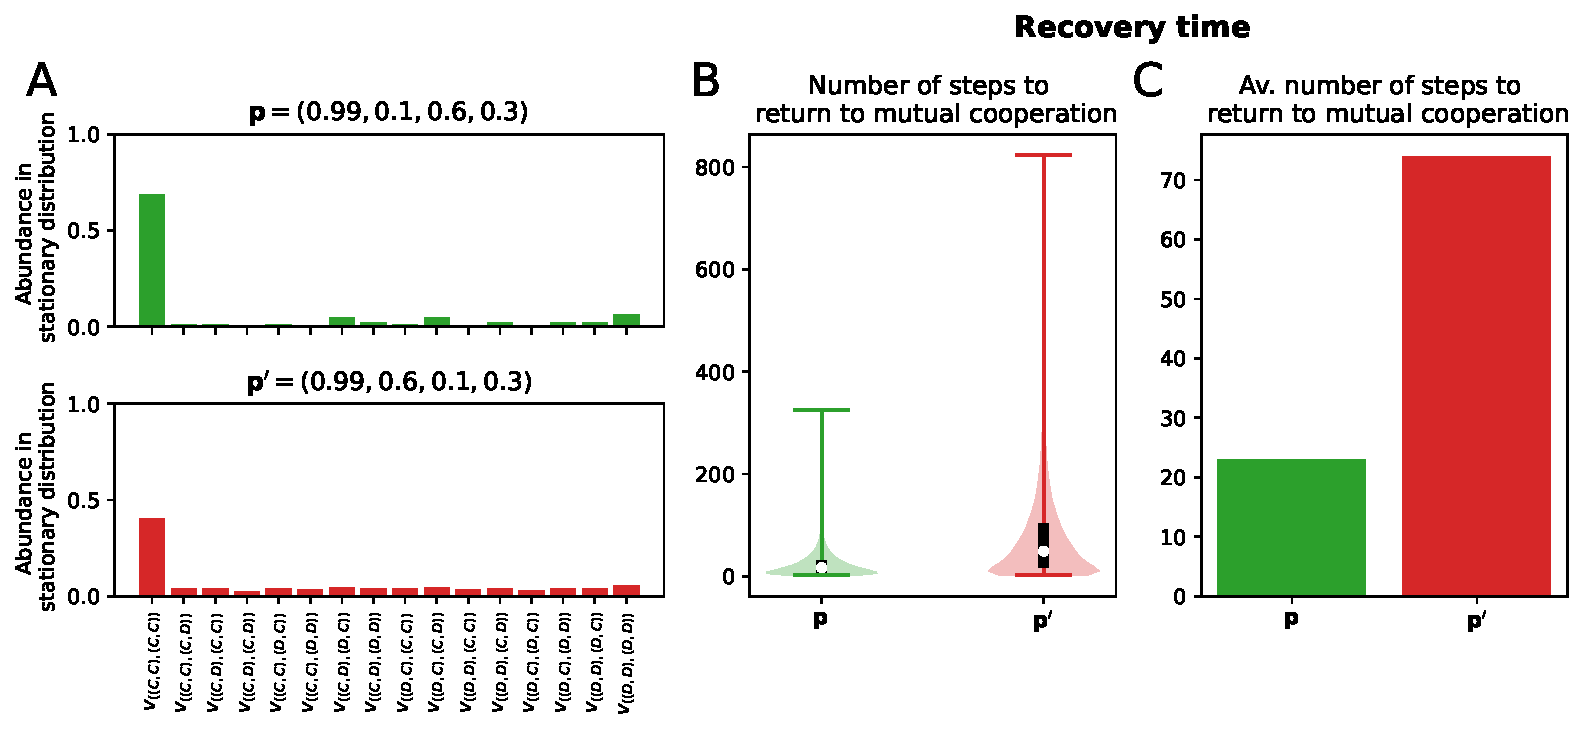
\includegraphics[width=\textwidth]{../../figures/siFigReactiveTwoPayoffs.pdf}
  \caption{\textbf{The difference between \(\mathbf{p}\) and \(\mathbf{p'}\) when
  \(p_{CC}, p'_{CC} \neq 1\).}
  The self-payoffs \(\pi(\mathbf{p}, \mathbf{p})\) and \(\pi(\mathbf{p'},
  \mathbf{p'})\) would be equal if the strategies were nice, more specifically if
  \(p_{CC} = p'_{CC} = 1\). However, such strategies are never
  sampled in the evolutionary process. For each mutant we introduce, we sample
  each element of the mutant from a uniform distribution. This means that the
  probability of sampling a strategy with \(p_{CC} = 1\) is zero.
  To understand the difference between the two strategies, we
  calculate the stationary distribution of the self-play of \(\mathbf{p}\) and \(\mathbf{p'}\). The
  stationary distribution shows us that the strategy \(\mathbf{p}\) spends significantly
  more time in the \(((C, C), (C, C))\) state than \(\mathbf{p'}\), which explains the
  difference in their payoffs.
  To explore where this difference arises, we conduct the following analysis: we
  assume a pair of players, playing either as \(\mathbf{p}\) or
  \(\mathbf{p'}\), starting in the \(((C, C), (C, D))\) state, which represents
  mutual cooperation with the second player defecting. We then calculate the
  expected time it takes for the strategies to return to the \(((C, C), (C, C))\)
  state. This is done by simulating the interactions using the Axelrod-Python~\cite{AxelrodPython}
  package and recording the number of actions/turns required to return to the
  \(((C, C), (C, C))\) state. We refer to this number as the recovery time. We repeat
  this process \(5 \times 10^4\) times for each pair of strategies. We plot the
  distribution of recovery times for both strategies in {\bf B} and the average
  recovery time for each strategy in {\bf C}. We observe that \(\mathbf{p}\)
  requires significantly fewer steps, on average, to return to the \(((C, C), (C, C))\) state
  than \(\mathbf{p'}\).}\label{fig:ReactiveTwoPayoffs}
\end{figure}



\begin{table}
  \centering
  \resizebox{\textwidth}{!}{
  \begin{tabular}{c|rlccc|rlccc}
    \toprule
    & \multicolumn{5}{c}{$\mathbf{p} = (0.99,0.1, 0.6, 0.3)$} &  \multicolumn{5}{c}{$\mathbf{p'} = (0.99, 0.6, 0.1, 0.3)$} \\
    \toprule
    \thead{Most common \\ paths} &   & Path &  \thead{Recovery \\ time} & Path probability & \thead{Frequency of occurrence \\ in $5 \times 10^4$ simulations} & & Path &   \thead{Recovery \\ time} & Path probability&  \thead{Frequency of occurrence \\ in $5 \times 10^4$ simulations}\\
    \midrule
    1  &  \cellcolor{gray!25} \makecell[r]{CC \\ CD} & \makecell[l]{     CC \\       CC} &  2 &  0.0588 & 5.9\%  &   \cellcolor{gray!25} \makecell[r]{CC \\ CD} & \makecell[l]{           CC \\            CC} &   2 &   0.0588 & 5.9\% \\ \hline
    2  &  \cellcolor{gray!25} \makecell[r]{CC \\ CD} & \makecell[l]{    DCC \\      CCC} &  3 &  0.0318 & 3.0\%  &   \cellcolor{gray!25} \makecell[r]{CC \\ CD} & \makecell[l]{         CDCC \\          CCCC} &   4 &   0.0311 & 3.2\% \\ \hline
    3  &  \cellcolor{gray!25} \makecell[r]{CC \\ CD} & \makecell[l]{   DCCC \\     CDCC} &  4 &  0.0171 & 1.8\%  &   \cellcolor{gray!25} \makecell[r]{CC \\ CD} & \makecell[l]{       CDCCCC \\        CCCDCC} &   6 &   0.0165 & 1.6\% \\ \hline
    4  &  \cellcolor{gray!25} \makecell[r]{CC \\ CD} & \makecell[l]{  DCDCC \\    CDCCC} &  5 &  0.0093 & 1.0\%  &   \cellcolor{gray!25} \makecell[r]{CC \\ CD} & \makecell[l]{     CDCCCDCC \\      CCCDCCCC} &   8 &   0.0087 & 0.9\% \\ \hline
    5  &  \cellcolor{gray!25} \makecell[r]{CC \\ CD} & \makecell[l]{  DDDCC \\    CDCCC} &  5 &  0.0093 & 0.9\%  &   \cellcolor{gray!25} \makecell[r]{CC \\ CD} & \makecell[l]{         DDCC \\          CCCC} &   4 &   0.0063 & 0.6\% \\ \hline
    6  &  \cellcolor{gray!25} \makecell[r]{CC \\ CD} & \makecell[l]{   DDCC \\     CCCC} &  4 &  0.0063 & 0.6\%  &   \cellcolor{gray!25} \makecell[r]{CC \\ CD} & \makecell[l]{   CDCCCDCCCC \\    CCCDCCCDCC} &  10 &   0.0046 & 0.4\% \\ \hline
    7  &  \cellcolor{gray!25} \makecell[r]{CC \\ CD} & \makecell[l]{  DDDCC \\    CDDCC} &  5 &  0.0065 & 0.6\%  &   \cellcolor{gray!25} \makecell[r]{CC \\ CD} & \makecell[l]{       DDCCCC \\        CCCDCC} &   6 &   0.0033 & 0.3\% \\ \hline
    8  &  \cellcolor{gray!25} \makecell[r]{CC \\ CD} & \makecell[l]{ DCDCCC \\   CDDDCC} &  6 &  0.0050 & 0.5\%  &   \cellcolor{gray!25} \makecell[r]{CC \\ CD} & \makecell[l]{       CDCCCC \\        CCDDCC} &   6 &   0.0033 & 0.3\% \\ \hline
    9  &  \cellcolor{gray!25} \makecell[r]{CC \\ CD} & \makecell[l]{ DCDCCC \\   CDCDCC} &  6 &  0.0050 & 0.5\%  &   \cellcolor{gray!25} \makecell[r]{CC \\ CD} & \makecell[l]{       DDCCCC \\        CCDDCC} &   6 &   0.0024 & 0.2\% \\ \hline
    10 &  \cellcolor{gray!25} \makecell[r]{CC \\ CD} & \makecell[l]{ DDDDCC \\   CDDCCC} &  6 &  0.0045 & 0.4\%  &   \cellcolor{gray!25} \makecell[r]{CC \\ CD} & \makecell[l]{          DCC \\           CCC} &   3 &   0.0024 & 0.2\% \\ \hline
    11 &  \cellcolor{gray!25} \makecell[r]{CC \\ CD} & \makecell[l]{ DDDCCC \\   CDDDCC} &  6 &  0.0045 & 0.4\%  &   \cellcolor{gray!25} \makecell[r]{CC \\ CD} & \makecell[l]{ CDCCCDCCCDCC \\  CCCDCCCDCCCC} &  12 &   0.0024 & 0.2\% \\ \hline
    12 &  \cellcolor{gray!25} \makecell[r]{CC \\ CD} & \makecell[l]{ DCDDCC \\   CDDDCC} &  6 &  0.0035 & 0.4\%  &   \cellcolor{gray!25} \makecell[r]{CC \\ CD} & \makecell[l]{     CDCCCDCC \\      CCDDCCCC} &   8 &   0.0018 & 0.2\% \\ \hline
    13 &  \cellcolor{gray!25} \makecell[r]{CC \\ CD} & \makecell[l]{   DDCC \\     CDCC} &  4 &  0.0035 & 0.3\%  &   \cellcolor{gray!25} \makecell[r]{CC \\ CD} & \makecell[l]{     CDCCDDCC \\      CCCDCCCC} &   8 &   0.0018 & 0.2\% \\ \hline
    14 &  \cellcolor{gray!25} \makecell[r]{CC \\ CD} & \makecell[l]{ DDDDCC \\   CDDDCC} &  6 &  0.0032 & 0.3\%  &   \cellcolor{gray!25} \makecell[r]{CC \\ CD} & \makecell[l]{     DDCCCDCC \\      CCCDCCCC} &   8 &   0.0018 & 0.2\% \\ \hline
    15 &  \cellcolor{gray!25} \makecell[r]{CC \\ CD} & \makecell[l]{DCDCDCC \\  CDCDCCC} &  7 &  0.0020 & 0.3\%  &   \cellcolor{gray!25} \makecell[r]{CC \\ CD} & \makecell[l]{        DCCCC \\         CCDCC} &   5 &   0.001 & 0.1\% \\  \hline
    Sum & & &  &  & 16.9\% & & & &  & 14.5\% \\
    \bottomrule
    \end{tabular}}
    \caption{We have used the Axelrod-Python~\cite{AxelrodPython} package to simulate interactions between two players. First, both players used the strategy \(\mathbf{p} = (0.99, 0.10, 0.60, 0.30)\), and then they used the strategy \(\mathbf{p'} = (0.99, 0.60, 0.10, 0.30)\). We assumed that the players start by both cooperating, followed by the second player defecting, resulting in the history \( ((C, C), (C, D)) \). We recorded not only the time it took to return to \( ((C, C), (C, C)) \) but also the sequence of actions taken by the two players. Here, we present the most common paths taken by the players in both cases.
    The paths are shown in the ``Path'' column, as well as the recovery time, and their frequency of occurrence. We can observe that the most common path is the same for both strategies, where following a defection by player 2, both players cooperate twice in a row to return to the state of mutual cooperation. For the rest of the most common paths, we can quickly observe that the recovery times of those paths are shorter in the case of \(\mathbf{p}\) than in the case of \(\mathbf{p'}\).
    In the case of \(\mathbf{p'}\), two of the most common paths have a recovery time longer than 10, whereas in the case of \(\mathbf{p}\), the longest recovery time is 7.}
\end{table}

% %%%%%%%%%%%%
% %% Errors  %%
% %%%%%%%%%%%%

\clearpage

\section{Errors}

So far, we have considered the case where there cannot be a mistake in the
actions taken by a player; the actions of the players are realized without
error. Here, we discuss what happens in the case where such an error is
possible. More specifically, we consider that \(\epsilon\) is the probability
that a player makes a mistake in the action taken.

\begin{figure}[h]
    \centering
    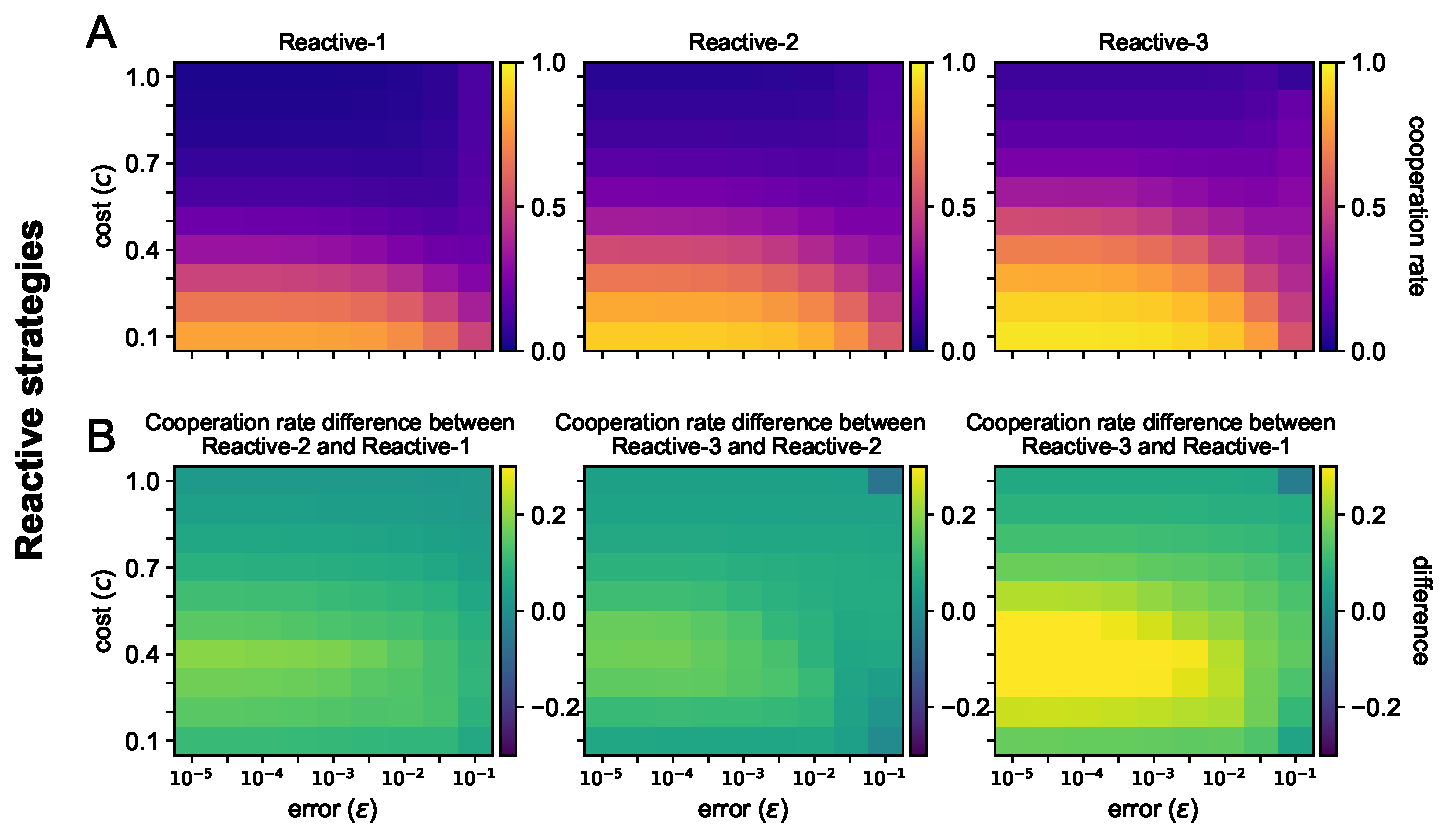
\includegraphics[width=.65\textwidth]{../../figures/siFig2Errors.pdf} \\[2em]
    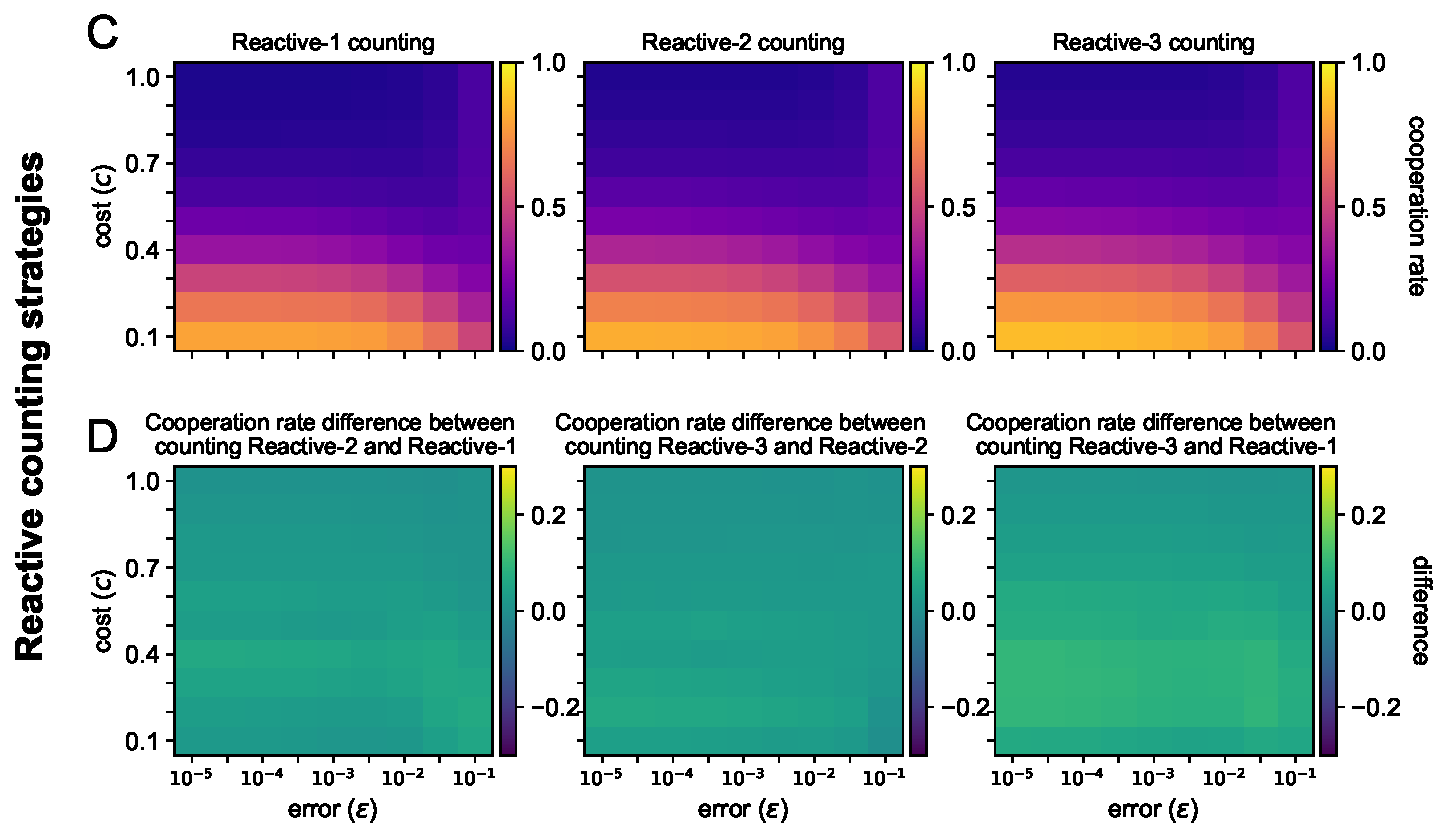
\includegraphics[width=.65\textwidth]{../../figures/siFigErrorsCounting.pdf}
    \caption{
    \textbf{Cooperation rates with implementation errors.}
  We simulate the evolutionary process, this time allowing for implementation
  errors. Specifically, we consider a probability \(\epsilon\) that a player makes
  a mistake in the action taken. We calculate the average cooperation rate for
  different values of \(\epsilon\) and \(c\). We do this for reactive strategies
  {\bf A} and reactive counting strategies {\bf C}. {\bf A, C,} We plot the average
  cooperation rate for the different parameters when individuals use reactive-1,
  reactive-2, and reactive-3 strategies, respectively. {\bf B, D,} We plot the
  differences between the cooperation rates when individuals use different memory
  size strategies. From left to right, we show the differences between reactive-1
  and reactive-2, reactive-2 and reactive-3, and reactive-1 and reactive-3
  strategies.
    }\label{fig:errors}
\end{figure}


% %%%%%%%%%%%%
% %% Memory-n  %%
% %%%%%%%%%%%%


\newpage

\section{Memory-$n$}

So far in the evolutionary simulations, we have considered reactive strategies
and demonstrated that strategies with larger memory capacities lead to more
cooperative populations. We now repeat the evolutionary simulations, but this
time using memory-$n$ strategies. We obtain results for memory-$1$, memory-$2$,
and memory-counting strategies, with $n$ equal to $1$, $2$, and $3$. Memory-$n$
counting strategies are a subset of memory-$n$ strategies, where players only
respond to the number of past cooperations between the two players, ignoring the
exact timing of cooperation.

A memory-$n$ strategy can be represented as a vector $\mathbf{m} = (m_{i,j})$,
with $0 \leq i, j \leq n$. The entries $m_{i,j}$ denote a player's probability
of cooperating in the next round, given that the focal player has cooperated $i$
times in the last $n$ rounds, while the co-player has cooperated $j$ times.
Similarly to reactive strategies for \(n = 1\), the two spaces are the same.

The main result still holds. For more memory, more cooperation evolves, however,
not in the case of counting strategies.


\begin{figure}[h]
  \centering
  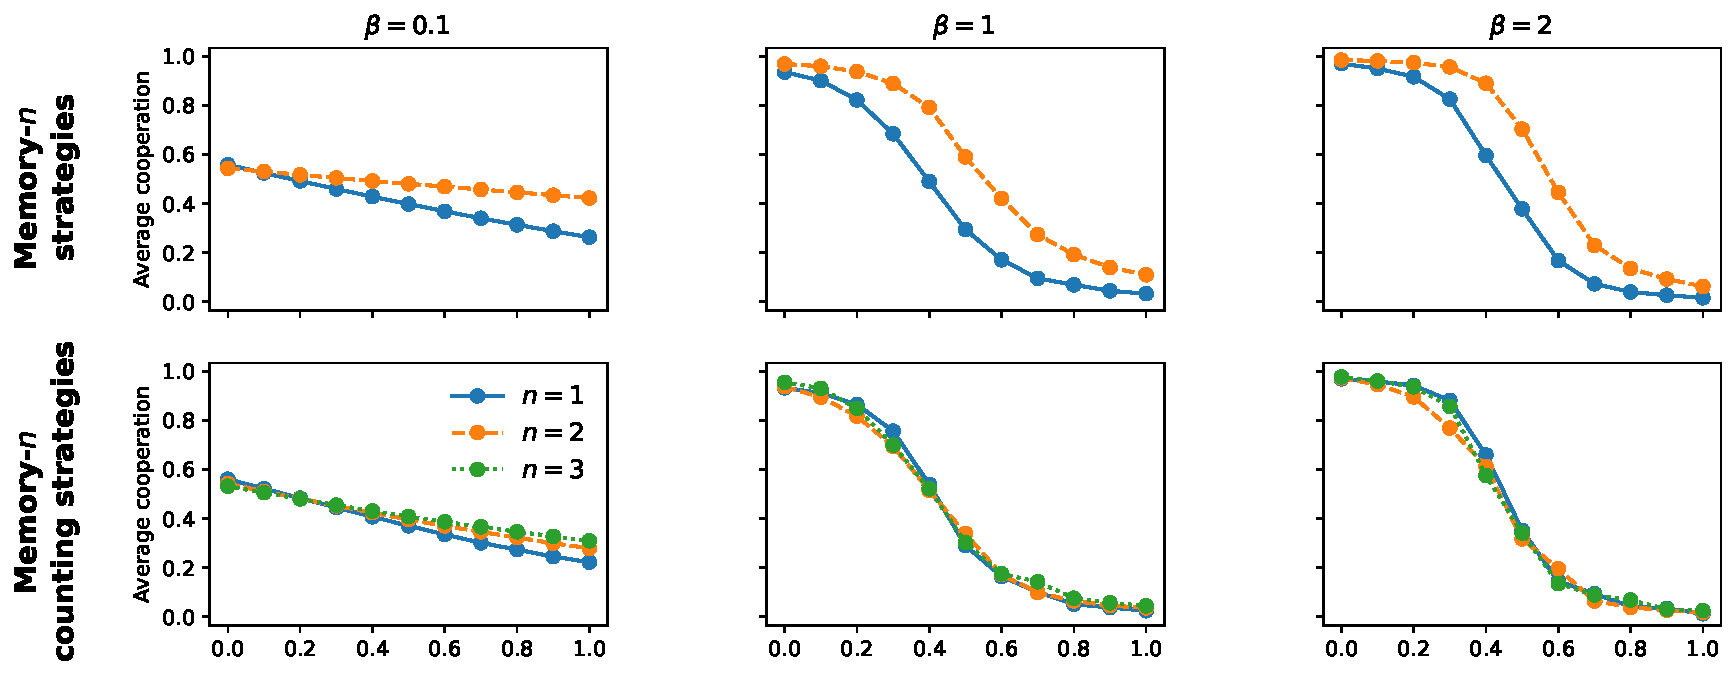
\includegraphics[width=.75\textwidth]{../../figures/siFigMemorySim.pdf}
  \caption{
  \textbf{Memory-$n$ simulations.}
  We explore the cooperation rates of memory-$n$ strategies and memory-$n$
  counting strategies over different values of cost and selection strength.
  Simulations are based on a donation game with \(b\!=\!1\),  \(c\!=\!0.5\), a
  selection strength $\beta\!=\!1$ and a population size $N\!=\!100$, unless
  noted otherwise. For $n$ equal to 1 and 2, simulations are run for \(T\!=\! 10
  ^ 7\) time steps.
  }
\end{figure}


\begin{figure}[h]
  \centering
  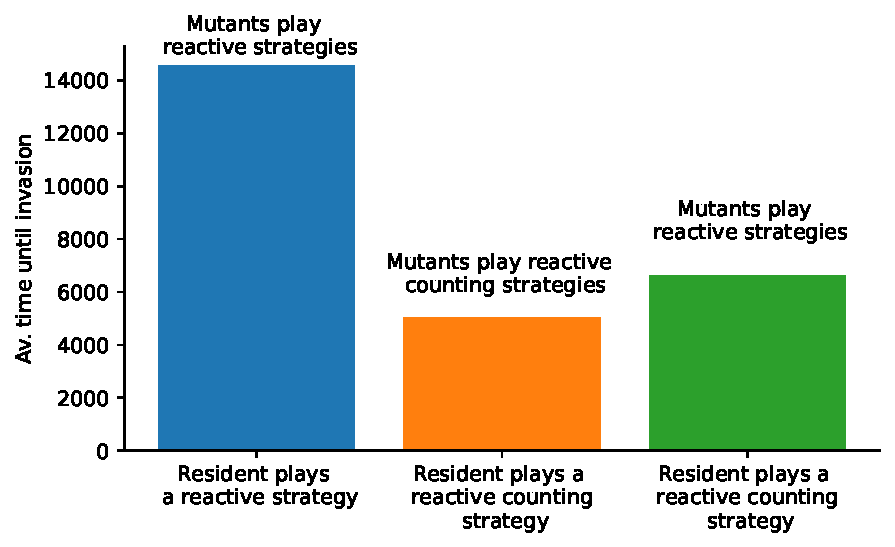
\includegraphics[width=.45\textwidth]{../../figures/siFigCountingReactiveInvasionTime.pdf}
  \caption{{\bf Invasion times for reactive and reactive counting.}
  To understand why counting strategies do not allow for more cooperation, we
  focus on reactive-2 strategies and reactive-2 counting strategies. For
  \(\beta=1\) and \(c=0.3\), what we observe is that the top abundant strategies
  for both simulations are very cooperative strategies, achieving a cooperation
  rate of \(\approx 1\). From the top strategies, it is also clear that the
  average time until they were invaded is higher for reactive strategies. To test
  this, we perform the following exercise: we pick a top abundant reactive
  strategy and a reactive counting strategy. These are (0.999985, 0.160136,
  0.553336, 0.035629) for the reactive strategy and (0.998204, 0.466715, 0.317605)
  for the reactive counting strategy. We run an invasion analysis when both
  strategies are residents. For the reactive counting strategy, we run two
  invasion analyses: one where only counting reactive mutants are introduced and
  one with reactive mutants. What we observe is that the reactive strategy can
  repel more mutants. However, we also see that for the counting strategy, when we
  consider reactive mutants, the average time until invasion increases. We run
  \(10^3\) simulations and take the average.}
\end{figure}



\newpage
\section{Proofs}

%%%%%%%%%%%%%%%%%%%%%%%%%%%%%%
%%  PROOFS:  Reactive-1 defective Nash, donation game  %%
%%%%%%%%%%%%%%%%%%%%%%%%%%%%%%

\subsection{Proof of Theorem~\ref{theorem:reactive_one_defecting_strategies}:
Reactive-1 defective Nash strategies in the donation game}
\begin{proof}
The proof is similar to one for partner strategies. We again enumerate the four
pure self-reactive-1 strategies  $\mathbf{\tilde p}$  by interpreting the
strategy as a binary number, we obtain the following payoffs.

\begin{equation*}\label{Eq:PayoffExpressionsDefectiveReactiveOne}
  \begin{array}{lcll}
   \pi^1(\mathbf{\tilde p_j},\mathbf{p}) &= &\displaystyle 0 & ~~\text{for}~ j\! \in\!  \{0, 2\} \\[0.3cm]
   \pi^1(\mathbf{\tilde p_j},\mathbf{p}) &= &\displaystyle  \frac{b \cdot p_{C} - c}{p_{C} + 1}  & ~~\text{for}~ j\! \in\!  \{1\} \\[0.3cm]
   \pi^1(\mathbf{\tilde p_j},\mathbf{p}) &= &\displaystyle  b \cdot p_{c} - c  & ~~\text{for}~ j\! \in\!  \{3\} \\[0.3cm]
  \end{array}
\end{equation*}

Requiring the payoffs in this list to be at most the mutual defection payoff $0$, we get the following unique conditions,
\begin{equation*}
 p_{D}  \le \frac{c}{b}.
\end{equation*}
\end{proof}

%%%%%%%%%%%%%%%%%%%%%%%%%%%%%%
%%  PROOFS:  Reactive-2 defective Nash, donation game  %%
%%%%%%%%%%%%%%%%%%%%%%%%%%%%%%


\subsection{Proof of Theorem~\ref{theorem:reactive_two_defecting_strategies}:
Reactive-2 defective Nash strategies in the donation game}
\begin{proof}
The proof is similar to one for partner strategies. We again enumerate the sixteen
pure self-reactive-2 strategies  $\mathbf{\tilde p}$  by interpreting the
strategy as a binary number, we obtain the following payoffs.

\begin{equation*}\label{Eq:PayoffExpressionsDefectiveReactiveTwo}
  \begin{array}{lcll}
   \pi^1(\mathbf{\tilde p_j},\mathbf{p}) &= &\displaystyle 0 & ~~\text{for}~ j\! \in\!  \{0, 2, 4, 6, 8, 10, 12, 14\} \\[0.3cm]
   \pi^1(\mathbf{\tilde p_j},\mathbf{p}) &= &\displaystyle  \frac{p_{CD} + p_{DC}}{3}\,b - \frac{c}{3}  & ~~\text{for}~ j\! \in\!  \{1, 9\} \\[0.3cm]
   \pi^1(\mathbf{\tilde p_j},\mathbf{p}) &= &\displaystyle  \frac{p_{CC} + p_{CD} + p_{DC}}{4}\,b - \frac{c}{2} & ~~\text{for}~ j\! \in\!  \{3\} \\[0.3cm]
   \pi^1(\mathbf{\tilde p_j},\mathbf{p}) &= &\displaystyle  \frac{p_{CD} + p_{DC}}{2}\,b - \frac{c}{2}  & ~~\text{for}~ j\! \in\!  \{4, 5, 12, 13\} \\[0.3cm]
   \pi^1(\mathbf{\tilde p_j},\mathbf{p}) &= &\displaystyle  \frac{p_{CC} + p_{CD} + p_{DC}}{3}\,b - \frac{2 c}{3}  & ~~\text{for}~ j\! \in\!  \{6, 7\}\\[0.3cm]
   \pi^1(\mathbf{\tilde p_j},\mathbf{p}) &= &\displaystyle  p_{CC}\,b - c & ~~\text{for}~ j\! \in\!  \{8, 9, 10, 11, 12, 13, 14, 15\}
  \end{array}
\end{equation*}

Requiring the payoffs in this list to be at most the mutual defection payoff $0$, we get the following unique conditions,
\begin{equation*}
  p_{CC}  \le \frac{c}{b}, \qquad \qquad
 \frac{p_{CD} + p_{DC}}{2}  \le \frac{1}{2} \cdot  \frac{c}{b}, \qquad \qquad
  \frac{p_{CD} + p_{DC} + p_{CC}}{3} \le	\frac{2}{3} \cdot \frac{c}{b}.
 \end{equation*}
Because the last condition is implied by the first two, we end up with the
conditions in~\eqref{eq:defecting_conditions_two}. 
\end{proof}


%%%%%%%%%%%%%%%%%%%%%%%%%%%%%%
%%  PROOFS:  Reactive-3 defective Nash, donation game  %%
%%%%%%%%%%%%%%%%%%%%%%%%%%%%%%

\subsection{Proof of Theorem~\ref{theorem:reactive_three_defecting_strategies}:
Reactive-3 defective Nash strategies in the donation game}

\begin{proof}
  The proof is similar to the previous one. 
  Again, enumerating the 256 pure self-reactive 3 strategies $\mathbf{\tilde p}$ by interpreting the strategy as a binary number, we obtain the following payoffs. 
  \begin{equation*}\label{Eq:PayoffExpressionsReactiveThree}
  \footnotesize
  \setlength{\arraycolsep}{0mm}
  \begin{array}{lclll}
  \pi^1(\mathbf{\tilde p_j},\mathbf{p}) &{\, = \,}
  &\displaystyle 0
  &~\text{for}~ j\! \in\! 
  &\{0, 2, 4, 6, \dots, 250, 252, 254\} \\[0.2cm]
  
  \pi^1(\mathbf{\tilde p_j},\mathbf{p}) &= 
  &\displaystyle \frac{p_{CDD} + p_{DCD} + p_{DDC}}{4} \,b - \frac{1}{4} \,c
  &~\text{for}~ j\! \in\!  
  & \{ 1, 9, 33, 41, 65, 73, 97, 105, 129, 137, 161,
    \\ & & &  &169, 193, 201, 225, 233\} \\[0.2cm]
      
  \pi^1(\mathbf{\tilde p_j},\mathbf{p}) &= 
  &\displaystyle \frac{p_{CCD} + p_{CDD} + p_{DCC} + p_{DDC}}{5}\, b - \frac{2}{5} \,c
  &~\text{for}~ j\! \in\!  
  & \{ 3, 7, 35, 39, 131, 135, 163, 167\} \\[0.2cm]
  
  \pi^1(\mathbf{\tilde p_j},\mathbf{p}) &= 
  &\displaystyle \frac{p_{CDC} + p_{DCD}}{2} \, b - \frac{1}{2} \, c
  &~\text{for}~ j\! \in\!  
  & \{ 4 \!- \!7, 12 \!- \!15, 20 \!- \!23, 28 \!- \!31, 68 \!- \!71,
      \\ & & &  &76 \!- \!79, 84 \!- \!87, 92 \!- \!95, 132 \!- \!135, 
      \\ & & & &140 \!- \!143, 148- 151, 156 \!- \!159, 
      \\ & & & &196 \!- \!199, 204 \!- \!207, 212 \!- \!215, 220 \!- \!223\} \\[0.2cm]
      
  \pi^1(\mathbf{\tilde p_j},\mathbf{p}) &= 
  &\displaystyle \frac{p_{CCC} + p_{CCD} + p_{CDD} + p_{DCC} + p_{DDC}}{6} \,b - \frac{1}{2} \, c
  &~\text{for}~ j\! \in\! 
  & \{ 11, 15, 43, 47\} \\ [0.2cm]
  
  \pi^1(\mathbf{\tilde p_j},\mathbf{p}) &= 
  &\displaystyle \frac{p_{CDD} + p_{DCD} + p_{DDC}}{3} \, b - \frac{1}{3} \, c
  &~\text{for}~ j\! \in\! 
  & \{16,17,24,25,48,49,56,57,80,81,88,
      \\ & & & &89,112, 113,120,121, 144,145,152,153,
      \\ & & & &176,177,184,185,208,209,216,217,
      \\ & & & &240, 241,248,249\} \\[0.2cm]
      
  \pi^1(\mathbf{\tilde p_j},\mathbf{p}) &= 
  &\displaystyle \frac{p_{CCD} + p_{CDD} + p_{DCC} + p_{DDC}}{4} \, b - \frac{1}{2} \, c
  &~\text{for}~ j\! \in\! 
  & \{ 18, 19, 22, 23, 50, 51, 54, 55, 146, 147,
      \\ & & &  &150, 151, 178, 179, 182, 183\} \\[0.2cm]
      
  \pi^1(\mathbf{\tilde p_j},\mathbf{p}) &= 
  &\displaystyle \frac{p_{CCC} + p_{CCD} + p_{CDD} + p_{DCC} + p_{DDC}}{5} \, b - \frac{3}{5} \, c
  &~\text{for}~ j\! \in\! 
  & \{ 26, 27, 30, 31, 58, 59, 62, 63\} \\ [0.2cm]
  
  \pi^1(\mathbf{\tilde p_j},\mathbf{p}) &= 
  &\displaystyle \frac{p_{CCD} + p_{CDC} + p_{CDD} + p_{DCC} + p_{DCD} + p_{DDC}}{7}\, b - \frac{3}{7} \, c
  &~\text{for}~ j\! \in\! 
  & \{ 37, 67, 165, 195\} \\ [0.2cm]
  
  \pi^1(\mathbf{\tilde p_j},\mathbf{p}) &= 
  &\displaystyle \frac{p_{CCC} + p_{CCD} + p_{CDC} + p_{CDD} + p_{DCC} + p_{DCD} + p_{DDC}}{8} \, b - \frac{1}{2} \, c ~~~~~
  &~\text{for}~ j\! \in\! 
  & \{ 45, 75\} \\ [0.2cm]
  
  \pi^1(\mathbf{\tilde p_j},\mathbf{p}) &= 
  &\displaystyle \frac{p_{CCD}+ p_{CDC}+ p_{CDD}+ p_{DCC}+ p_{DCD}+ p_{DDC}}{6} \, b - \frac{1}{2} \, c
  &~\text{for}~ j\! \in\! 
  & \{ 52, 53, 82, 83, 180, 181, 210, 211\} \\  [0.2cm]
  
  \pi^1(\mathbf{\tilde p_j},\mathbf{p}) &= 
  &\displaystyle \frac{p_{CCC} + p_{CCD} + p_{CDC} + p_{CDD} + p_{DCC} + p_{DCD} + p_{DDC}}{7} \, b - \frac{4}{7} \, c
  &~\text{for}~ j\! \in\! 
  & \{ 60, 61, 90, 91\} \\ [0.2cm]
  
  \pi^1(\mathbf{\tilde p_j},\mathbf{p}) &= 
  &\displaystyle \frac{p_{CCD} + p_{CDC} + p_{DCC}}{3} \, b - \frac{2}{3} \, c
  &~\text{for}~ j\! \in\! 
  & \{ 96\!- \!103, 112\!- \!119, 224\!- \!231, 240\!- \!247\} \\ [0.2cm]
      
  \pi^1(\mathbf{\tilde p_j},\mathbf{p}) &= 
  &\displaystyle \frac{p_{CCC} + p_{CCD} + p_{CDC} + p_{DCC}}{4} \, b - \frac{3}{4} \, c
  &~\text{for}~ j\! \in\! 
  & \{ 104\!-\!111, 120\!- \!127\} \\ [0.2cm]
  
  \pi^1(\mathbf{\tilde p_j},\mathbf{p}) &= 
  &\displaystyle p_{CCC} \, b - c
  &~\text{for}~ j\! \in\! 
  & \{128, 129, 130, \dots, 255\}
  \end{array}
  \end{equation*}
  
  \noindent
  Requiring these payoffs to be at most  equal to the mutual defection payoff 0
  gives

  \begin{equation*} \footnotesize
  \begin{array}{c}
  \displaystyle  p_{CCC} \leq \frac{c}{b}, 
    \qquad \qquad \frac{p_{CDC} + p_{DCD}}{2} \leq \frac{1}{2} \cdot \frac{c}{b}, 
    \qquad \qquad \frac{p_{CDD} + p_{DCD} + p_{DDC}}{3} \leq \frac{1}{3} \cdot \frac{c}{b},\\[0.45cm]
  \displaystyle  \frac{p_{CCD} + p_{CDC} + p_{DCC}}{3} \leq \frac{2}{3} \cdot \frac{c}{b},
    \quad \qquad \frac{p_{CCD} + p_{CDD} + p_{DCC} + p_{DDC}}{4} \leq \frac{1}{2}  \cdot \frac{c}{b}, \\[0.45cm]
    \displaystyle  \frac{p_{CCC} + p_{CCD} + p_{CDC} + p_{DCC}}{4} \leq \frac{3}{4} \cdot \frac{c}{b},
    \quad \qquad \frac{p_{CCC} + p_{CCD} + p_{CDD} + p_{DCC} + p_{DDC}}{6} \leq \frac{1}{2}  \cdot \frac{c}{b}, \\[0.45cm]
    \displaystyle  \frac{p_{CCD} + p_{CDC} + p_{CDD} + p_{DCC} + p_{DCD} + p_{DDC}}{6} \leq \frac{1}{2}  \cdot \frac{c}{b},
    \quad \qquad \frac{p_{CCC} + p_{CCD} + p_{CDC} +  p_{CDD} + p_{DCC} +  p_{DCD} + p_{DDC}}{8} \leq \frac{1}{2}  \cdot \frac{c}{b}.
    \end{array}
  \end{equation*}

  \noindent
  The statement follows by noting that the five conditions in the first two rows imply the four other conditions.
\end{proof}
 
{\setlength{\bibsep}{0\baselineskip}
\bibliographystyle{naturemag}
\bibliography{../../bibliography.bib}
}

\end{document}